% Inline bibliography: compile twice with pdflatex, or use latexmk -bibtex- -pdf.
% Preserve the modern LaTeX label before REVTeX installs its legacy version.
\let\SavedKernelLabel\label
\documentclass[aps,pra,reprint,amsmath,amssymb,longbibliography,floatfix]{revtex4-2}
\usepackage[T1]{fontenc}
\usepackage[utf8]{inputenc}
\usepackage{bm}
\usepackage{amsthm}
\usepackage{graphicx}
\usepackage{tikz}
\usepackage{pgfplots}
\usepackage{booktabs}
\usepackage{microtype}
% Hyperref expects the modern kernel label with current LaTeX releases.
\makeatletter
\@ifl@t@r\fmtversion{2023-06-01}{\let\label\SavedKernelLabel\let\ltx@label\label}{}
\makeatother
\usepackage[hidelinks]{hyperref}
\usetikzlibrary{arrows.meta,positioning,calc,fit,backgrounds,patterns}
\usepgfplotslibrary{fillbetween}
\pgfplotsset{compat=1.18}
\newtheorem{theorem}{Theorem}
\newtheorem{proposition}[theorem]{Proposition}
\newcommand{\tr}{\operatorname{tr}}
\newcommand{\id}{\operatorname{id}}
\newcommand{\sinc}{\operatorname{sinc}}
\newcommand{\norm}[1]{\lVert#1\rVert}
\newcommand{\ket}[1]{\lvert#1\rangle}
\newcommand{\bra}[1]{\langle#1\rvert}
\newcommand{\DV}{\mathcal D_V}
\newcommand{\wt}[1]{\widetilde{#1}}
\begin{document}
\title{Mechanical mediation through shared apparatus in gravitational-entanglement experiments}
\author{Samuel Mausberg}
\affiliation{Independent Researcher}
\date{October 3, 2026}
\begin{abstract}
Can the support shared by two matter-wave interferometers entangle their path-recording spins, even when its final motion records neither path? It can. For prescribed forces coupled to a linear Gaussian apparatus, we bound the resulting spin channel by two force-weighted cross responses. Classical force replay measures the bound; local pulse changes can null both responses. For passive mounts, finite-time bounds on static compliances cover every mechanical mode, and a spectral gap gives a controlled elastic approximation. When gravity acts mainly during a hold, the permissible pulse-weighted compliance scales as the cube of the ramp time. A specified clamped horizontal link produces a phase comparable to a millisecond-ramp gravitational reference, but negligible for long ramps. These results provide a calibration criterion for excluding a mechanical entangling channel, rather than a contamination estimate for an uncharacterized instrument.
\end{abstract}
\maketitle
\raggedbottom

\section{Introduction}
The apparatus that splits a matter wave receives a reaction force. If two interferometers use the same support, can that support generate the entanglement intended to witness gravity? It can, even when its final motion contains no record of either path. The relevant experimental question is therefore how much of this additional channel survives the actual force sequence. This paper answers it through a force-to-displacement cross response, rather than an assigned recoil mass or an assumed fringe visibility. The internal two-state systems that record the paths will be called the records.

For a linear Gaussian apparatus, two pulse-weighted cross responses bound the entire mechanical record channel. They can be measured by replaying amplified classical forces at the same work-conjugate ports. Nulling both responses removes the entangling part by changing local controls. We also derive a conservative passive-mount certificate from static compliances, including all modes. These three results turn the mechanical background into an acceptance test with explicit constants.

Rapid splitting makes the test more demanding. For a stiff response and a fixed gravitational holding time, the allowed pulse-weighted compliance falls as the cube of the ramp time. The test mass and splitting amplitude cancel from the leading phase ratio. Thus small superpositions alone are not the problem; the potentially costly choice is preparing them rapidly while allowing little time for gravity to act. A specified horizontal elastic link illustrates this distinction without identifying a vertical table mode with an unknown interferometer cross response.

The original proposals by Bose et al.\ and Marletto and Vedral require other entangling interactions to be excluded or bounded \cite{Bose,Marletto}. Apparatus effects have since been studied from several directions. Danielson, Satishchandran, and Wald include the compensating laboratory dipole \cite{Danielson}. C\'eleri, Soares-Pinto, and Vanzella analyze recoil during preparation, recoverable coherence, and acoustic limits on the participating apparatus \cite{Celeri}. Gunnink et al.\ calculate gravitational entanglement with heavy apparatus oscillators \cite{Gunnink}. Casimir-screening analyses include surface forces and bound branch-dependent plate deflection and its effect on path coherence \cite{Kamp,Schut}. Williams's constrained-motion proposal assumes independent mechanical supports \cite{Williams}.

Elahi et al.\ propose a shared-apparatus geometry in which two nanodiamonds are trapped on opposite sides of a microfabricated chip \cite{Elahi}. They identify vibrational noise transmitted through the chip's mechanical supports and discuss possible isolation strategies. A detailed noise analysis and the design of the Stern-Gerlach pulse sequence remain for future work. Their proposal does not quantify entanglement mediated by the chip's branch-dependent elastic response. Once the relevant force sequence is specified, the criterion derived here applies to that response.

Neither the coherent bus mechanism nor the Gaussian solution is new. Motional gates can return a thermally occupied bus while entangling the controlled systems \cite{Molmer}; multiqubit Gaussian noise spectroscopy already relates quantum cross spectra, pulse filters, and induced couplings \cite{PazSilva}. Our contribution is the channel-distance certificate, its classical force-replay and nulling rules, and finite-time compliance bounds tied to interferometer forces. The result does not require reconstructing the whole noise spectrum.

We carry the nominal long-pulse geometry of Bose et al.\ through the calculation. Its test-pair phase is $-0.3612$ rad for the smooth pulse specified below. We then compare its compliance requirement with a short-ramp completion of a constrained geometry. The comparison distinguishes a published geometry, a chosen pulse, and a specified mounting model throughout.

\section{From closed recoil to a measured response}
\subsection{Why coherent return is insufficient}
A simple exactly soluble case isolates the effect before any mounting approximation is made. Two test bodies of masses $m_A,m_B$ receive forces $z_i a_i(t)$ from a common free support of mass $M$, where $z_i=\pm1$ is the eigenvalue of the record's Pauli operator $Z_i$. Their positions are $x_i$, the support position is $X$, and their canonical momenta are $p_i,P$. Consider
\begin{equation}
H_0=\sum_{i=A,B}\frac{p_i^2}{2m_i}+\frac{P^2}{2M}-\sum_{i=A,B}Z_i a_i(t)(x_i-X).
\label{eq:freeH}
\end{equation}
The force and reaction sum to zero. Let $d_i(t)$ be the full inertial branch separation, so that $a_i=m_i\ddot d_i/2$. Assume $d_i=\dot d_i=0$ at both ends of the cycle. Up to global and local record phases, the final unitary is
\begin{equation}
\begin{split}
U(T)&=U_{\rm free}(T)e^{i\Delta_{\rm rec}Z_AZ_B/4},\\
\Delta_{\rm rec}&=-\frac{m_A m_B}{M\hbar}\int_0^T\dot d_A(t)\dot d_B(t)\,dt.
\end{split}
\label{eq:recoil}
\end{equation}
This factorization holds for every initial motional state. It follows because linear-force commutators are scalars: the Magnus expansion stops at second order, closure removes displacement operators, and two integrations by parts give Eq.~\eqref{eq:recoil}. Appendix~\ref{app:free} gives the proof and a causal elastic completion.

The support displacement can be tiny while its phase is appreciable. It equals
\begin{equation}
X_z-X_{\rm free}=-\frac{m_Az_A d_A+m_Bz_Bd_B}{2M}.
\label{eq:displacement}
\end{equation}
For initial $\ket{++}$, with each $+$ an $X$ eigenstate, the ideal record negativity is $|\sin(\Delta_{\rm rec}/2)|/2$. The free-ended elastic model in Appendix~\ref{app:free} gives negativity above $0.49998$ with gravity absent. Its error bound includes every mode, so the example does not rely on an instantaneous rigid propagator.

Equation~\eqref{eq:recoil} also gives an exact special-purpose control: nonoverlapping branch velocities cancel free translation. A mounted apparatus can remember earlier forces, so that control need not cancel its full channel. We now replace the free mass by its measurable response.

\subsection{Force ports and model assumptions}
The two record operators commute. A mechanical port coordinate $q_i$ is defined by work: an applied force $F_i$ contributes $-F_iq_i$ to the Hamiltonian. For an extended actuator, $q_i$ is the displacement averaged against its actual force distribution. After branch-independent forces are included in the reference trajectory, the interaction is
\begin{equation}
H_I(t)=-Z_A f_A(t)q_A(t)-Z_B f_B(t)q_B(t).
\label{eq:HI}
\end{equation}
Here $f_i$ is half the difference between the two forces on the apparatus. For Eq.~\eqref{eq:freeH}, $f_i=-a_i$. Multiple force locations and directions are retained by replacing each product by a vector contraction; the two record labels do not change.

The loads must be obtained from the branch-dependent interaction, not from the test body's acceleration alone. For prescribed paths with interaction energies $U_{i,+}$ and $U_{i,-}$, a retained apparatus coordinate $q_\alpha$ has load $f_{i\alpha}= -\tfrac12\partial_{q_\alpha}(U_{i,+}-U_{i,-})$ at the reference configuration. In a magnetic splitter this includes the reaction on the field sources and their supports. Confining forces can also load an anchor during a hold. Forces at different locations, and torques with their conjugate angles, must be kept separately even when their resultant vanishes.

We assume quadratic dynamics for the apparatus together with its damping reservoir, linear canonical port observables, and an initially Gaussian state of all these traced-out degrees of freedom, independent of the records and any spectator. The forces are prescribed nondemolition controls, meaning that they do not change the record labels, and all smeared covariances converge. We subtract the mean port motion and calibrate the resulting local record phases. These assumptions allow a continuum of modes, correlated fluctuations, memory, and time-dependent linear dynamics. Neither weak coupling nor a Markov approximation is required.

\begin{figure}[t]
\centering
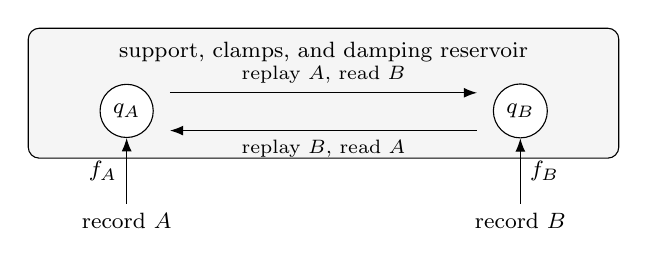
\begin{tikzpicture}[x=1cm,y=1cm,>=Latex,font=\footnotesize]
\draw[rounded corners,fill=black!4] (0,0) rectangle (7.5,1.65);
\node at (3.75,1.35) {support, clamps, and damping reservoir};
\node[draw,circle,fill=white,inner sep=3pt] (a) at (1.25,.6) {$q_A$};
\node[draw,circle,fill=white,inner sep=3pt] (b) at (6.25,.6) {$q_B$};
\node (ra) at (1.25,-.8) {record $A$};
\node (rb) at (6.25,-.8) {record $B$};
\draw[->] (ra) -- node[left] {$f_A$} (a);
\draw[->] (rb) -- node[right] {$f_B$} (b);
\draw[->] (1.8,.83) -- node[above,font=\scriptsize] {replay $A$, read $B$} (5.7,.83);
\draw[<-] (1.8,.35) -- node[below,font=\scriptsize] {replay $B$, read $A$} (5.7,.35);
\end{tikzpicture}
\caption{The relevant mechanical connection is measured at the actual force distributions. Both directed actions integrate the observed cross displacement against the other interferometer's force. Material stiffness, damping, and attachment to a frame enter through this response.}
\label{fig:ports}
\end{figure}

Since the commutator is a scalar, the retarded response is
\begin{equation}
\chi_{ij}(t,s)=\frac{i}{\hbar}\vartheta(t-s)[q_i(t),q_j(s)],
\label{eq:chi}
\end{equation}
where $\vartheta$ is the Heaviside function. It is also the exact change of mean displacement per classical applied force. A seismic transmissibility, relating base displacement to table displacement, is not this response. Nor is displacement at an arbitrary pickup necessarily the work-conjugate $q_i$.

Define the two directed cross actions
\begin{equation}
I_{ij}=\int_0^T f_i(t)\int_0^t\chi_{ij}(t,s)f_j(s)\,ds\,dt,\qquad i\ne j.
\label{eq:actions}
\end{equation}
Their sum and difference determine distinct phases in the record channel:
\begin{equation}
\Delta_m=\frac{2(I_{AB}+I_{BA})}{\hbar},\qquad
\sigma=\frac{I_{AB}-I_{BA}}{2\hbar}.
\label{eq:phases}
\end{equation}
The first is a coherent $Z_AZ_B$ phase. The second appears in the reservoir overlap between different record histories. Reciprocity of the stationary response does not make the two actions equal for unequal pulse timings.

\subsection{A bound on the complete record channel}
A phase fit alone cannot distinguish an entangling response from correlated noise. To make that distinction, set
\begin{equation}
Q_i=\hbar^{-1}\int_0^T f_i(t)q_i(t)\,dt,\qquad
V_{ij}=\tfrac12\langle Q_iQ_j+Q_jQ_i\rangle.
\label{eq:V}
\end{equation}
Let $\DV$ average the product unitary $e^{i(\xi_AZ_A+\xi_BZ_B)}$ over a centered classical Gaussian variable $\xi$ of covariance $V$. This channel can erase coherence but cannot entangle separable records.

\begin{theorem}[Response certificate]
Under the assumptions above, the final mechanical record channel $\Phi$ satisfies, for every input state $\rho$ and any spectator system,
\begin{equation}
D\bigl((\Phi\otimes\id)(\rho),(\DV\otimes\id)(\rho)\bigr)\le\beta,
\label{eq:certificate}
\end{equation}
\begin{equation}
\beta=\min\left\{1,\frac{\max(|I_{AB}|,|I_{BA}|)}{\hbar}\right\}.
\label{eq:beta}
\end{equation}
Here $D(\rho,\rho')=\norm{\rho-\rho'}_1/2$. No value of $V$ is needed to evaluate the bound.
\end{theorem}

The proof in Appendix~\ref{app:channel} keeps both phases in Eq.~\eqref{eq:phases}. It scales the quantum couplings by $\sqrt u$ and adds classical local rotations with covariance $(1-u)V$. The noise stays fixed while the response phases scale by $u$. Every intermediate map is completely positive. Integrating its trace-distance derivative gives $|\Delta_m|/4+|\sigma|=\max(|I_{AB}|,|I_{BA}|)/\hbar$. The constant is sharp to first order for a noiseless closed bus gate.

This result supplies an operational mechanical-only null. For a fixed sign $s=\pm1$, the witness
\begin{equation}
W_s=\frac{I-X_AX_B+s(Y_AZ_B+Z_AY_B)}4
\label{eq:witness}
\end{equation}
has nonnegative expectation on separable states and spectral range one. Thus initially separable records, with gravity and other entangling channels absent, obey
\begin{equation}
-\tr\bigl(W_s\Phi(\rho_{\rm sep})\bigr)\le\beta.
\label{eq:falsepositive}
\end{equation}
For comparison, $e^{i\Delta_g Z_AZ_B/4}\ket{++}$ gives
\begin{equation}
w_g=\frac{|\sin(\Delta_g/2)|}{2}
\label{eq:wg}
\end{equation}
with the matching sign. Allocating a fraction $\eta$ of this ideal signal to mechanics means requiring $\beta\le\eta w_g$. This bounds a false positive; it does not assume that the ideal signal survives noise.

\section{Calibration and local removal}
\subsection{Replay the force, not the seismic disturbance}
The channel certificate becomes useful when the same actions can be measured without resolving a single branch's minute displacement. Apply an amplified force $\lambda_j f_j$ at port $j$, with the other branch-dependent force off, and measure the baseline-subtracted cross displacement $y_{i\leftarrow j}$. The apparatus configuration, controller setting, and spatial force profile are unchanged. Linearity gives
\begin{equation}
\widehat I_{ij}=\frac1{\lambda_j}\int_0^T f_i(t)y_{i\leftarrow j}(t)\,dt.
\label{eq:replay}
\end{equation}
The gain is admissible only over a verified linear range. Increasing a splitter's current does not by itself implement this replay: it can change the trap stiffness or the force distribution. The calibrated drive must reproduce the differential load, including any retained force and torque components.

The norms below are time-domain $L^p$ norms. If the complete displacement error satisfies $\norm{\delta y_{ij}}_\infty\le\delta y_{ij}^{\max}$, H\"older's inequality gives
\begin{equation}
\begin{split}
e_{ij}&=\frac{\norm{f_i}_1\delta y_{ij}^{\max}}{|\lambda_j|},\\
\beta_{\rm cal}&=\min\left\{1,\frac{\max_{i\ne j}(|\widehat I_{ij}|+e_{ij})}{\hbar}\right\}.
\end{split}
\label{eq:calerror}
\end{equation}
For an $L^2$ displacement-error bound $\epsilon_{ij}$, use
\begin{equation}
e_{ij}=\norm{f_i}_2\epsilon_{ij}/|\lambda_j|.
\label{eq:l2error}
\end{equation}
The error includes baseline subtraction, gain, drift, sensor bandwidth, and admitted departure from linearity. Appendix~\ref{app:replay} adds force-waveform errors and finite-sample witness uncertainty. A finite measured frequency band cannot silently replace an all-frequency response.

For the running example we choose the smooth opening profile
\begin{equation}
d(t)=d_0s(t/\tau),\qquad s(u)=35u^4-84u^5+70u^6-20u^7,
\label{eq:pulse}
\end{equation}
followed by a hold of duration $H$ and the reversed closing ramp. The source geometry and nominal ramp and hold times follow the explicit scheme of Ref.~\cite{Bose}
\begin{equation}
\begin{gathered}
m=10^{-14}\ {\rm kg},\quad R=450\ \mu{\rm m},\quad d_0=250\ \mu{\rm m},\\
\tau=0.5\ {\rm s},\qquad H=2.5\ {\rm s}.
\end{gathered}
\label{eq:boseinputs}
\end{equation}
The polynomial is our endpoint-smooth replacement for the proposal's idealized acceleration sequence. It gives $f=-m\ddot d/2$, $\norm f_1=2.1875\times10^{-17}\ {\rm N\,s}$, and the test-pair Newtonian phase $\Delta_g=-0.3611838$ rad, including both ramps.

As a specified acceptance target, take $\lambda=10^{11}$ and a complete raw displacement-error bound $0.1$ nm. The peak replay force is $3.76\ \mu{\rm N}$ and $e/\hbar\simeq2.07430\times10^{-4}$. A specified $400$ kg free translating capsule gives $\Delta_{\rm rec}=-9.6704\times10^{-4}$ rad. If replay returns these actions, Eq.~\eqref{eq:calerror} gives $\beta_{\rm cal}<4.50\times10^{-4}$, below $0.01w_g=8.98\times10^{-4}$. The capsule calculation isolates translation; the replay test, not its nominal mass, must cover the remaining response.

\subsection{Cancel both directed actions}
Calibration can also specify a control change instead of merely accepting a background. For a fixed apparatus response, hold $f_A$ fixed and change the other local force to
\begin{equation}
f_B=f_{B0}+a_1g_1+a_2g_2,\qquad
\int g_\ell\,dt=\int t g_\ell\,dt=0.
\label{eq:loops}
\end{equation}
The added loops preserve inertial displacement and momentum closure. Let $b$ contain the two baseline actions, and let column $\ell$ of $C$ contain the two actions with $g_\ell$ in place of $f_B$.

\begin{proposition}[Two-response null]
If $C$ is invertible, $a=-C^{-1}b$ makes the final mechanical channel exactly $\DV$, with $V$ evaluated for the modified forces. With measured coefficients, choose $a=-\widehat C^{-1}\widehat b$. If their entrywise action errors are $e_{b,r}$ and $e_{C,r\ell}$, then
\begin{equation}
\beta_{\rm null}\le\min\left\{1,\frac1\hbar\max_r\left(e_{b,r}+\sum_{\ell=1}^2|a_\ell|e_{C,r\ell}\right)\right\}.
\label{eq:nullerror}
\end{equation}
\end{proposition}

Both actions are linear in $f_B$. Their residual is $b+Ca$, proving the exact statement and, by a rowwise triangle inequality, the error bound. This is a change of local pulses, not subtraction of an entangling gate from measured data. Correlated dephasing may remain; the null does not preserve its original covariance.

A numerical example in Appendix~\ref{app:replay} uses a damped test response and the Bose pulse. Simply delaying one interferometer by $0.5$ s nulls free recoil but not its two damped actions. Two added loops remove both while retaining $86.5\%$ of the original test-pair gravitational phase. The coefficients are bounded and the corrected branch separation remains between zero and $d_0$. This example illustrates conditioning and pulse closure, rather than assigning the test response to an actual horizontal mount.

\section{Passive compliance and rapid preparation}
\subsection{A measurable design rule}
A useful comparison between pulse families should not depend on a guessed platform mass. For nonzero forces, define the pulse-weighted cross compliance
\begin{equation}
\bar\chi_{ij}=\frac{I_{ij}}{\norm{f_i}_2\norm{f_j}_2}.
\label{eq:weightedchi}
\end{equation}
It has units of m/N and retains the phase cancellations in the actual waveform, for stationary or nonstationary response. Equation~\eqref{eq:beta} gives the sufficient, directly testable requirement
\begin{equation}
\max_{i\ne j}|\bar\chi_{ij}|\le\frac{\eta\hbar w_g}{\norm{f_A}_2\norm{f_B}_2}.
\label{eq:budget}
\end{equation}
For stationary response, a uniform bound $|\chi_{ij}(\omega)|\le\chi_*$ implies $|\bar\chi_{ij}|\le\chi_*$ by Parseval and Cauchy--Schwarz, but replay is usually less conservative and does not infer a uniform envelope from finitely many samples.

For identical collinear pulses with $d_0<R$, the exact pair reference is
\begin{equation}
\Delta_g=-\frac{2Gm^2}{\hbar R^3}\int_0^T\frac{d(t)^2}{1-d(t)^2/R^2}\,dt.
\label{eq:gravity}
\end{equation}
Define $H_{\rm eff}=H+1042\tau/1287$ for Eq.~\eqref{eq:pulse}. Its force norm is
\begin{equation}
\norm f_2^2=\frac{140m^2d_0^2}{11\tau^3}.
\label{eq:forcenorm}
\end{equation}
For reciprocal response and these identical pulses, the common $\bar\chi$ gives $\Delta_m=4\bar\chi\norm f_2^2/\hbar$. Bounding the denominator in Eq.~\eqref{eq:gravity} yields the exact interval
\begin{equation}
\begin{gathered}
(1-d_0^2/R^2)\mathcal R\le\left|\frac{\Delta_m}{\Delta_g}\right|\le\mathcal R,\\
\mathcal R=\frac{280|\bar\chi|R^3}{11G\tau^3 H_{\rm eff}}.
\end{gathered}
\label{eq:ratio}
\end{equation}
The susceptibility itself changes when the pulse changes. A nearly static stiff response gives a $\tau^{-3}$ phase ratio for a hold-dominated cycle; free translation instead gives $\tau^{-1}$. Equation~\eqref{eq:ratio} separates this mechanical dispersion from the kinematic pulse cost. There is no enhancement caused by reducing $m$ or $d_0$ alone at leading small splitting.

\begin{table}[t]
\caption{Maximum pulse-weighted cross compliance from Eq.~\eqref{eq:budget} for a one-percent ideal-witness budget. Thresholds are rounded downward. The smooth pulse is a design choice in every row; the two short ramp times are not specified by Ref.~\cite{Williams}.}
\label{tab:budget}
\begin{ruledtabular}
\begin{tabular}{lccc}
Reference & $\tau$ (s) & $w_g$ & bound (m/N)\\
Bose \cite{Bose} & $0.5$ & $8.981\times10^{-2}$ & $1.48\times10^{-4}$\\
Screened \cite{Schut} & $0.25$ & $2.375\times10^{-2}$ & $3.65\times10^{-4}$\\
Short, 1 ms & $0.001$ & $4.456\times10^{-6}$ & $3.69\times10^{-12}$\\
Short, 10 ms & $0.01$ & $4.687\times10^{-6}$ & $3.88\times10^{-9}$
\end{tabular}
\end{ruledtabular}
\end{table}

Table~\ref{tab:budget} lists acceptance thresholds, not inferred hardware properties. The screened reference uses the published surface-force trajectory, not a fixed initial gap. The short-ramp rows use Williams's mass, spacing, and splitting with our explicit ramp and hold completion. Their holding trajectories are fixed by control, not identified with an unforced pendulum orbit. The input models and phase derivations are given in Appendix~\ref{app:gravity}.

\subsection{All-mode bounds from passive mechanics}
A static compliance is not a uniform frequency-response bound: a lightly damped resonance can exceed it. The following finite-time estimate avoids that substitution. Assume a stationary reciprocal passive response with a real oscillator representation
\begin{equation}
\chi_{ij}(t)=\vartheta(t)\sum_n\frac{c_{ni}c_{nj}}{M_n\omega_n}\sin(\omega_nt),\qquad M_n,\omega_n>0.
\label{eq:modes}
\end{equation}
A convergent positive spectral measure may replace the sum, including the loss reservoir. Let the static self compliances be finite:
\begin{equation}
C_i=\sum_n\frac{c_{ni}^2}{M_n\omega_n^2},\qquad
C_{ij}=\sum_n\frac{c_{ni}c_{nj}}{M_n\omega_n^2}.
\label{eq:compliances}
\end{equation}
Free zero modes must be separated before using these quantities.

\begin{theorem}[Finite-time passive compliance]
For absolutely continuous compact forces with integrable derivatives,
\begin{equation}
|I_{ij}|\le\sqrt{C_iC_j}\bigl(\norm{f_i}_2\norm{f_j}_2+\norm{f_i}_1\norm{\dot f_j}_1\bigr).
\label{eq:passive}
\end{equation}
If all response modes also satisfy $\omega_n\ge\omega_1>0$, and the zero-extended forces have absolutely continuous first derivatives and integrable second derivatives, then
\begin{equation}
\begin{split}
\left|I_{ij}-C_{ij}\int f_if_j\,dt\right|&\le E_{ij},\\
E_{ij}=\frac{\sqrt{C_iC_j}}{\omega_1^2}\bigl[&\norm{\dot f_i}_2\norm{\dot f_j}_2
+\norm{\dot f_i}_1\norm{\ddot f_j}_1\bigr].
\end{split}
\label{eq:gap}
\end{equation}
\end{theorem}

The first estimate is an all-mode design certificate even when a resonance lies inside the pulse spectrum. It assumes no gap and no lower bound on damping. The second gives a controlled static approximation when a gap is known, without discarding a high-frequency pulse tail. Appendix~\ref{app:passive} proves both by integration by parts and a spectral Cauchy--Schwarz inequality. Combining either with Eq.~\eqref{eq:beta} turns a justified compliance measurement or model into a mechanical witness budget.

\subsection{A horizontal mounting model}
To test whether fast-pulse sensitivity requires a freely moving kilogram, consider an explicitly clamped longitudinal elastic link. Its displacement field $u(x)$ on $0<x<\ell$ has Hamiltonian
\begin{equation}
H_R=\frac12\int_0^\ell\left[\frac{\pi(x)^2}{\varrho A}+EA(\partial_xu)^2\right]dx.
\label{eq:rodH}
\end{equation}
The endpoints obey $u(0)=u(\ell)=0$. Here $E$ is Young's modulus, $\varrho$ is mass density, $A$ is cross-sectional area, and $\pi$ is momentum per unit length. The two horizontal axial force profiles are uniform patches of width $b$, centered at $\ell/3$ and $2\ell/3$. The model is local with wave speed $c_s=\sqrt{E/\varrho}$ and first frequency $\omega_1=\pi c_s/\ell$.

We choose $\ell=0.10$ m, $A=10^{-4}\ {\rm m^2}$, $b=10^{-3}$ m, and nominal density $\varrho=8000\ {\rm kg/m^3}$ as design inputs. NIST's 304-stainless modulus fit at 293 K gives $E=199.534$ GPa \cite{NISTsteel}. The link mass is $0.080$ kg and $\omega_1/(2\pi)=24.971$ kHz. The force patches specify the attachment of the actuators, not the spacing of the test masses.

The exact patch-averaged static Green function gives
\begin{equation}
\begin{split}
C_{AB}&=\frac{\ell}{9EA}=5.56854\times10^{-10}\ {\rm m/N},\\
C_A=C_B&=\frac{2\ell/9-b/6}{EA}=1.10536\times10^{-9}\ {\rm m/N}.
\end{split}
\label{eq:rodC}
\end{equation}
For Eq.~\eqref{eq:boseinputs}, the static mechanical phase is only $1.3441\times10^{-8}$ rad, with an all-mode error below $2.99\times10^{-15}$ rad. A large freely translating mass was not needed to make that long-pulse background small.

For the short reference, take $m=10^{-14}$ kg, $R=100\ \mu{\rm m}$, $d_0=1\ \mu{\rm m}$, and $H=0.14$ s from the scales in Ref.~\cite{Williams}, but choose $\tau=1$ ms and actively held paths. Equation~\eqref{eq:gap} gives
\begin{equation}
2.538\times10^{-5}<\Delta_m<2.838\times10^{-5}\ {\rm rad}.
\label{eq:shortinterval}
\end{equation}
The pair reference is $-1.7825\times10^{-5}$ rad. The mechanical phase magnitude is therefore between $1.42$ and $1.60$ times that reference within the specified elastic model. The sign is opposite here; this is a coherent bias, not a claim that it reproduces every predicted gravitational correlator.

\begin{figure}[t]
\centering
\begin{tikzpicture}
\begin{loglogaxis}[width=.94\columnwidth,height=5.6cm,
 xlabel={Ramp time $\tau$ (ms)},ylabel={Compliance (m/N)},
 xmin=1,xmax=10,ymin=1e-12,ymax=1e-8,
 tick label style={font=\small},label style={font=\small},
 xtick={1,2,5,10},xticklabels={1,2,5,10},
 legend style={font=\scriptsize,draw=none,fill=none,at={(.03,.97)},anchor=north west},
 legend cell align=left,minor tick num=0]
\addplot[name path=lo,draw=none,forget plot] table[x=tau,y=lower]{compliance.dat};
\addplot[name path=hi,draw=none,forget plot] table[x=tau,y=upper]{compliance.dat};
\addplot[fill=black!22,draw=none] fill between[of=lo and hi];
\addlegendentry{All-mode enclosure}
\addplot[black,thick] table[x=tau,y=static]{compliance.dat};
\addlegendentry{Static link response}
\addplot[black,dashed,thick] table[x=tau,y=budget]{compliance.dat};
\addlegendentry{One-percent witness budget}
\end{loglogaxis}
\end{tikzpicture}
\caption{Design comparison for $R=100\ \mu{\rm m}$, $d_0=1\ \mu{\rm m}$, and $H=0.14$ s. The dashed curve is the measured-compliance acceptance threshold, not an assumed mount property. The band follows Eq.~\eqref{eq:gap} for the specified clamped link. Once its upper edge lies below the budget, all longitudinal modes meet the mechanical bound.}
\label{fig:compliance}
\end{figure}

Keeping the same link and hold but increasing the ramp to $10$ ms reduces the mechanical-to-gravitational phase ratio below $0.00144$. The corresponding bound is below one percent of the ideal witness. Figure~\ref{fig:compliance} shows the comparison as a compliance budget. A stiff horizontal load path can therefore require calibration for millisecond ramps, while longer ramps can satisfy a provable material-channel bound.

\subsection{Resolve the actual load path}
Constrained motion makes port identification especially important. In a linear pendulum model, $k=m\omega_p^2$ and a prescribed branch displacement $zd/2$ requires actuator force $zm(\ddot d+\omega_p^2d)/2$. The apparatus then receives two branch-dependent loads,
\begin{equation}
f_{\rm act}=-\frac m2(\ddot d+\omega_p^2d),\qquad
f_{\rm anchor}=\frac m2\omega_p^2d.
\label{eq:loads}
\end{equation}
Their sum is the inertial reaction $-m\ddot d/2$. Their mechanical work is not determined by that sum unless they act on the same displacement coordinate. Separated actuator and anchor motion requires the vector version of Eq.~\eqref{eq:actions}, including their cross responses. Appendix~\ref{app:passive} derives this statement and its coordinate invariance.

Williams's example uses $0.5$ m nanotube pendula and assumes independent supports; it supplies neither a complete reaction-force transfer matrix nor a ramp waveform \cite{Williams}. Accordingly, Eqs.~\eqref{eq:shortinterval} and \eqref{eq:loads} are a specified shared-mount completion and a calibration prescription, not a measured percentage for that proposal. Mechanical independence, when established as $\chi_{AB}=\chi_{BA}=0$ for every retained load component, is an exact null. A finite residual is handled by Eq.~\eqref{eq:calerror}.

\section{Discussion}
The source of concern is work done through a common quantum material response. Closing its trajectory does not remove the accumulated phase. Conversely, a sufficiently small pair of measured cross actions excludes a large mechanical entangling channel without requiring a mechanical visibility estimate. A complete two-response null removes that channel by local controls. These statements give a sharper experimental criterion than replacing a platform by a free mass or by the mass of the Earth.

The new design information is the finite-time compliance budget. Its passive version includes all response modes and does not assume that static stiffness bounds resonant amplification. Its gapped version makes the short-pulse elastic example controlled. The $\tau^{-3}$ stiff-response scaling explains why an apparatus adequate for a long interferometer may require a new calibration after the ramp is shortened.

The channel theorem assumes prescribed nondemolition forces, quadratic dynamics, and an initially Gaussian mechanical environment independent of the records. Branch-dependent stiffness, nonlinear control, autonomous actuator dynamics, and an unmodeled feedback path require separate bounds. The clamped link excludes bending, finite clamp compliance, and other load paths, all of which belong in a real replay measurement. Its geometry and density, the short ramps, and the replay accuracy are declared design choices; the modulus is a nominal material fit, not a certified sample value. A port-resolved load and susceptibility are needed to attribute a mechanical background to an actual instrument.

Coherent phase estimates alone do not predict observable entanglement. For example, the specified 293 K link with the 1 ms pulse has calculated $\tr V\simeq1.27\times10^{-3}$, which prevents the witness used here from detecting the much smaller coherent signal. Appendix~\ref{app:numerics} gives the covariance calculation and its mode-tail bound. Gravitational reference phases use prescribed Newtonian test-pair paths. Full apparatus gravity, controller stress, wave-packet dynamics, electromagnetic interactions, and detection errors remain separate budgets. None is set to zero by the mechanical certificate.

The distinction from previous work is correspondingly narrow. Reversible preparation recoil \cite{Celeri}, gravity-induced apparatus decoherence \cite{Gunnink}, branch-dependent screening-plate motion \cite{Kamp}, closed motional gates \cite{Molmer}, and quantum cross-spectrum reconstruction \cite{PazSilva} are established ingredients. The present bound retains the two directed actions as an operational channel-distance budget, and supplies classical replay, local nulling, and passive compliance estimates for that budget. Published vertical-heave data \cite{Hermsdorf} can motivate a numerical damping example but do not determine a horizontal cross response. We therefore do not use them to rank proposal families.

Finally, mechanical calibration does not depend on a gravitational gauge choice. It is defined by physical work and displacement. The complete Newtonian source has its own mixed branch terms when a recoil body is shared; Appendix~\ref{app:gravity} retains them and shows the cancellation of spurious support self-phases. For a conserved relativistic completion the usual gravitational Ward identity remains valid \cite{Danielson,Christodoulou}. Neither that identity nor a local gravitational description eliminates an additional material mediator. The experimental task is to bound both, rather than infer the absence of one from the coherent return of the other.

\begin{acknowledgments}
GPT-6 Astra Pro (OpenAI) assisted with calculations and manuscript preparation.
\end{acknowledgments}
\section*{Data availability}
The accompanying archive contains the complete \LaTeX\ source, calculation code, figure data, and tests. No experimental data were collected.

\appendix
\section{Exact Gaussian channel and response certificate}\label{app:channel}
Put $Q_z=z_AQ_A+z_BQ_B$. Scalar commutators make the Magnus expansion terminate, giving
\begin{equation}
 U_z=e^{i\theta_z}e^{iQ_z},\qquad
 \theta_z=\frac1{2\hbar}\sum_{ij}z_iz_jI_{ij}.
 \label{eq:Uz}
\end{equation}
The definition of $I_{ij}$ is extended to $i=j$ here. Such terms are global because $z_i^2=1$. Splitting the full-time commutator integral at $t=s$ gives
\begin{equation}
 [Q_A,Q_B]=-\frac{i}{\hbar}(I_{AB}-I_{BA}).
 \label{eq:commQ}
\end{equation}
Cyclicity of the reservoir trace, the Baker--Campbell--Hausdorff formula for scalar commutators, and the centered Gaussian characteristic function then give the exact record multiplier
\begin{align}
 \frac{\rho_{zz'}(T)}{\rho_{zz'}(0)}={}&
 \exp\left[\frac{i\Delta_m}{4}(z_Az_B-z'_Az'_B)\right]\nonumber\\
 &\times\exp[i\sigma(z_Az'_B-z_Bz'_A)]\nonumber\\
 &\times\exp[-\tfrac12(z-z')^TV(z-z')].
 \label{eq:channel}
\end{align}
The expression is interpreted as a Schur multiplier when an initial matrix element is zero. A coherent reservoir mean contributes only local phases. The same formula follows for convergent continuum covariances. Damping is represented by including its quadratic reservoir, not by replacing frequencies in a unitary propagator by complex numbers.

For $0\le u\le1$, scale the quantum forces by $\sqrt u$ and compose the resulting map with classical local Gaussian rotations of covariance $(1-u)V$, sampled independently of the reservoir. The total covariance stays $V$, while $\Delta_m,\sigma$ become $u\Delta_m,u\sigma$. This construction makes each interpolating map $\Phi_u$ completely positive and trace preserving, even on an input entangled with a spectator. Figure~\ref{fig:interpolation} records that construction.

\begin{figure}[t]
\centering
\begin{quantikz}[row sep=0.22cm,column sep=0.35cm]
\lstick{$A$}&\gate[3]{U_{\sqrt u}}&\gate{e^{i\xi_AZ_A}}&\qw\\
\lstick{$R$}& &\qw&\rstick{\text{trace}}\qw\\
\lstick{$B$}& &\gate{e^{i\xi_BZ_B}}&\qw
\end{quantikz}
\caption{A physical interpolation for the proof, not an experimental subtraction. Quantum couplings scale by $\sqrt u$; correlated classical rotations have covariance $(1-u)V$. Both noise contributions add to $V$.}
\label{fig:interpolation}
\end{figure}

For $X_u=(\Phi_u\otimes\id)(\rho)$, differentiation of Eq.~\eqref{eq:channel} gives
\begin{align}
 \partial_uX_u={}&\frac{i\Delta_m}{4}[Z_AZ_B,X_u]\nonumber\\
 &+i\sigma(Z_AX_uZ_B-Z_BX_uZ_A).
\end{align}
Identity operators on the spectator are implicit. Since $X_u$ is a density matrix and the Pauli factors are unitary,
\begin{equation}
 \tfrac12\norm{\partial_uX_u}_1\le |\Delta_m|/4+|\sigma|.
\end{equation}
Integrate over $u$ and use $(|a+b|+|a-b|)/2=\max(|a|,|b|)$ for real $a,b$. With $a=I_{AB}/\hbar$ and $b=I_{BA}/\hbar$, this proves Theorem~\ref{thm:response}. The cap follows from $D\le1$. For a closed noiseless gate, $V=0$, $\sigma=0$, and the distance on $|++\rangle$ is $|\sin(\Delta_m/4)|$, proving first-order sharpness.

For a product state with Bloch vectors $a,b$, four times the expectation of Eq.~\eqref{eq:witness} is $1-a_xb_x+s(a_yb_z+a_zb_y)$. Its bilinear term is $a^TK_sb$ for an orthogonal matrix $K_s$, hence is at least $-|a||b|\ge-1$. Convexity proves positivity on separable states. Direct Pauli multiplication gives spectrum $(-1/2,1/2,1/2,1/2)$, so
\begin{equation}
 |\tr[W_s(\rho-\rho')]|\le D(\rho,\rho').
\end{equation}
Combining this with Theorem~\ref{thm:response} proves Eq.~\eqref{eq:false}. The ideal-state correlators are $\langle XX\rangle=1$ and $\langle YZ\rangle=\langle ZY\rangle=-\sin(\Delta_g/2)$, proving Eq.~\eqref{eq:wg}.

The partial transpose of $W_s$ is the joint $+1$ stabilizer projector of $-X_AX_B$ and $sY_AZ_B$. These are commuting independent Pauli operators; the projector has rank one. Therefore $\mathcal N(\rho)\ge-\tr(W_s\rho)$, where negativity is the sum of absolute negative eigenvalues of $\rho^{T_B}$. This also proves the negativity estimates used below without identifying every witness violation with the exact negativity.

For reciprocal synchronous forces, $I_{AB}=I_{BA}$ and $\sigma=0$. Their mechanical overlap factors are
\begin{align}
 v_A&=e^{-2V_{AA}},\qquad v_B=e^{-2V_{BB}},\nonumber\\
 v_\pm&=e^{-2(V_{AA}+V_{BB}\pm2V_{AB})}.
\end{align}
On the initial $|++\rangle$, one obtains
\begin{equation}
 -\tr(W_s\rho)=\frac{v_++v_--2}{8}
       +\frac{v_A+v_B}{4}|\sin(\Delta_m/2)|
 \label{eq:visibility}
\end{equation}
for the matching sign. In particular, $\langle XX\rangle=(v_++v_-)/2$, not $v_Av_B$. The noise is correlated, and its value is derived from $V$ rather than assigned. If both cross actions vanish, Eq.~\eqref{eq:channel} reduces exactly to $\mathcal D_V$ for any physical $V$.

\section{Replay errors and the two-response control}\label{app:calibration}
A force $F_j$ changes the mean of $q_i$ by $\int\chi_{ij}F_j$. This follows by the linear Heisenberg equations, or by the first commutator in the Dyson series: its scalar value makes all further response commutators vanish. Equation~\eqref{eq:replay} and the H\"older error estimates therefore hold exactly in the stated model.

The actual force can also differ from its replay target. Write $f_i=\widehat f_i+\delta f_i$ and suppose $\norm{\delta f_i}_2\le r_i$. If the finite-window response has induced $L^2$ norm at most $K_{ij}$, and $\epsilon_{ij}$ bounds the nominal replay-displacement error in $L^2$, the action error is bounded by
\begin{align}
 e_{ij}\le{}&\frac{\norm{\widehat f_i}_2\epsilon_{ij}}{|\lambda_j|}\nonumber\\
 &+K_{ij}\left(r_i\norm{\widehat f_j}_2+
 r_j\norm{\widehat f_i}_2+r_ir_j\right).
 \label{eq:forceerror}
\end{align}
Expansion of the bilinear action and Cauchy--Schwarz prove all three additional terms. The response norm must itself be justified. This formula does not infer an unmeasured spectral tail from a few frequencies.

For stationary response, use the Fourier convention $\widetilde f(\omega)=\int f(t)e^{i\omega t}\dd t$ and extend forces by zero. Then
\begin{equation}
 I_{ij}=\int_{-\infty}^{\infty}\frac{\dd\omega}{2\pi}
 \widetilde f_i(\omega)^*\chi_{ij}(\omega)\widetilde f_j(\omega).
 \label{eq:Fourier}
\end{equation}
The integral is real. Absolute values and Cauchy--Schwarz prove the uniform-envelope assertion following Eq.~\eqref{eq:design}. Time-domain replay avoids needing such an envelope if its complete displacement error is already controlled.

The null of Proposition~\ref{prop:null} follows from $b+\mathsf C a=0$. With measured coefficients this residual is $(b-\widehat b)+(\mathsf C-\widehat{\mathsf C})a$, giving Eq.~\eqref{eq:nullerr}. Closure of a loop $g=-m\ddot d_g/2$ follows from $d_g=\dot d_g=0$ at its endpoints. Ill conditioning does not invalidate the identity, but can make its error bound or required force amplitudes unusable.

For an explicit numerical control, let $P_{\tau,H,t_0}$ denote the complete separation pulse of height $250\ \mu$m starting at $t_0$. Use
\begin{align}
 d_A&=P_{0.5,2.5,0},&d_{B0}&=P_{0.5,2.5,0.5},\nonumber\\
 d_{g_1}&=P_{0.25,0,0},&d_{g_2}&=P_{0.5,0,3}.
 \label{eq:loopdefs}
\end{align}
Choose the test susceptibility
\begin{gather}
 \chi(\omega)=\frac1{M(\Omega^2-\omega^2-2i\zeta\Omega\omega)},\nonumber\\
 M=187\ \mathrm{kg},\quad\Omega=2\pi(0.42\ \mathrm{Hz}),\quad\zeta=0.58.
 \label{eq:damped}
\end{gather}
These values come from the vertical-heave fit of Ref.~\cite{Hermsdorf}; here both port participations are a numerical design choice. They are not measured horizontal or constrained-device parameters. This response is used only to exhibit a nonsymmetric pair of actions and a well-conditioned null.

The baseline actions and control matrix are
\begin{align}
 b/\hbar&\simeq(-1.53613\times10^{-6},\ 1.79662\times10^{-4})^T,\nonumber\\
 \mathsf C/\hbar&\simeq10^{-4}
 \begin{pmatrix}
 1.64080465218&1.49297536559\\
 -1.63413864424&2.41243602167
 \end{pmatrix}.
\end{align}
The rounded coefficients are $a_1=0.42502996$ and $a_2=-0.45682594$. The first loop occurs before the delayed pulse, and the second subtracts from its final hold and closing ramp. Since $0<a_1<1$ and $-1<a_2<0$, direct comparison of the monotone opening and closing polynomials proves $0\le d_B\le d_0$. The retained gravitational phase is $86.5\%$ of the synchronized reference by the branch kernel in Appendix~\ref{app:gravity}.

\begin{figure}[t]
\centering
\begin{tikzpicture}
\begin{axis}[width=\columnwidth,height=5.1cm,
 xlabel={Time (s)},ylabel={Branch separation ($\mu$m)},
 xmin=0,xmax=4,ymin=-5,ymax=280,
 tick label style={font=\small},label style={font=\small},
 legend style={font=\footnotesize,at={(.5,.03)},anchor=south,draw=none}]
\addplot[black,dashed] table[x=t,y=A,col sep=comma]{../data/null_pulses.csv};\addlegendentry{$A$}
\addplot[black,dotted,thick] table[x=t,y=Bstaggered,col sep=comma]{../data/null_pulses.csv};\addlegendentry{Delayed $B$}
\addplot[black,thick] table[x=t,y=Bcorrected,col sep=comma]{../data/null_pulses.csv};\addlegendentry{Calibrated $B$}
\end{axis}
\end{tikzpicture}
\caption{The two-response null in the specified damped test model. Delaying $B$ removes the free-mode phase but not the mounted response. Two bounded closed loops cancel both directed actions while retaining a common gravitational interaction interval.}
\label{fig:null}
\end{figure}

An independent interval evaluation treats the nominal parameters in Eq.~\eqref{eq:damped} as exact. It gives
\begin{align}
 6.39806498735&<10^8\det(\mathsf C/\hbar)<6.39806498736,\nonumber\\
 -1.15405\times10^{-14}&<I_{AB}/\hbar<-1.15403\times10^{-14},\nonumber\\
 6.90469\times10^{-13}&<I_{BA}/\hbar<6.90471\times10^{-13}
\end{align}
for the eight-decimal coefficients, so $\beta<6.91\times10^{-13}$ is a numerical rounding bound for this test. More usefully, if each normalized response entry has measurement error at most $\epsilon$, Eq.~\eqref{eq:nullerr} gives $\beta_{\rm null}\le1.882\epsilon$ plus rounding error. Thus the residual is controlled by calibration, not by the displayed number of digits.

Finite witness statistics are separate. With $N$ independent trials for each of the three Pauli correlators and sign $s$ fixed in advance, Hoeffding's inequality and a union bound give witness error
\begin{equation}
 \epsilon_{\rm stat}=\frac34\sqrt{\frac{2\log(6/\alpha)}{N}}
\end{equation}
with probability at least $1-\alpha$. Each $[-1,1]$ correlator has error at most the square root except with probability $\alpha/3$. A violation exceeding $\beta_{\rm cal}+\epsilon_{\rm stat}$ rejects the covered mechanical-only null under these sampling assumptions. Established additional channel-distance errors add to that threshold.

\section{Passive compliance and the pulse scaling}\label{app:passive}
\subsection{Proof of the all-mode bounds}
Let $R_\omega(t)=\vartheta(t)\sin(\omega t)/\omega$ and define $J_\omega(g,f)=\int g(R_\omega*f)\dd t$. The forces are extended by zero. One integration by parts gives
\begin{equation}
 (R_\omega*f)(t)=\frac1{\omega^2}
 \left[f(t)-\int_{-\infty}^t\cos\omega(t-s)\dot f(s)\dd s\right].
 \label{eq:IBP}
\end{equation}
Consequently,
\begin{equation}
 |J_\omega(g,f)|\le\frac1{\omega^2}
 (\norm g_2\norm f_2+\norm g_1\norm{\dot f}_1).
 \label{eq:modebound}
\end{equation}
For each mode in Eq.~\eqref{eq:passive}, multiply by $|c_{ni}c_{nj}|/M_n$ and sum. The spectral Cauchy--Schwarz inequality
\begin{equation}
 \sum_n\frac{|c_{ni}c_{nj}|}{M_n\omega_n^2}
 \le\sqrt{C_iC_j}
\end{equation}
proves Eq.~\eqref{eq:passivebound}, also for a positive spectral measure. The finite right-hand side supplies domination for the continuum limit.

For the smoother forces of Eq.~\eqref{eq:staticerror}, $R_\omega''+\omega^2R_\omega=\delta$ and a second integration by parts give the exact identity
\begin{equation}
 J_\omega(g,f)=\frac{\langle g,f\rangle}{\omega^2}
                +\frac{J_\omega(\dot g,\dot f)}{\omega^2}.
 \label{eq:secondIBP}
\end{equation}
Indeed $R_\omega*f''=f-\omega^2R_\omega*f$ and
$\langle g,R_\omega*f''\rangle=-J_\omega(\dot g,\dot f)$; the zero-extended endpoint conditions remove boundary terms. Apply Eq.~\eqref{eq:modebound} to the last term and use
\begin{equation}
 \sum_n\frac{|c_{ni}c_{nj}|}{M_n\omega_n^4}
 \le\frac{\sqrt{C_iC_j}}{\omega_1^2}.
\end{equation}
This proves the second bound. No expansion in pulse bandwidth has been used. Replacing the full spectrum by a claimed gap is permissible only when the gap is actually part of the specified response model.

\subsection{Exact pulse constants}
Differentiating Eq.~\eqref{eq:pulse} gives $s'(u)=140u^3(1-u)^3$. Polynomial integration gives
\begin{align}
 \int_0^1(s')^2\dd u&=700/429,&
 \int_0^1(s'')^2\dd u&=280/11,\nonumber\\
 \int_0^1(s''')^2\dd u&=1120,&
 \int_0^1s^2\dd u&=521/1287.
\end{align}
For example, the first is $19600\,6!6!/13!$; the others follow by expanding the displayed polynomial. Splitting at the real roots of its successive derivatives gives
\begin{align}
 \int_0^1|s''|\dd u&=35/8,\nonumber\\
 \int_0^1|s'''|\dd u&=336\sqrt5/25,\nonumber\\
 \int_0^1|s''''|\dd u&=273.
\end{align}
The first is twice the maximum of $s'$. The extrema for the second occur at $u=(1\pm1/\sqrt5)/2$; those for the third occur at $u=1/2$ and $u=(1\pm\sqrt{3/5})/2$. Substitution in the preceding derivatives yields these absolute integrals. Both ramps therefore give
\begin{align}
 \norm f_1&=\frac{35md_0}{8\tau},&
 \norm f_2^2&=\frac{140m^2d_0^2}{11\tau^3},\nonumber\\
 \norm{\dot f}_1&=\frac{336\sqrt5\,md_0}{25\tau^2},&
 \norm{\dot f}_2^2&=\frac{560m^2d_0^2}{\tau^5},\nonumber\\
 \norm{\ddot f}_1&=\frac{273md_0}{\tau^3},&
 \max|f|&=\frac{42\sqrt5\,md_0}{25\tau^2}.
 \label{eq:norms}
\end{align}
The time integrals are
\begin{equation}
 \int\dot d^2\dd t=\frac{1400d_0^2}{429\tau},\qquad
 \int d^2\dd t=d_0^2\left(H+\frac{1042\tau}{1287}\right).
\end{equation}
These prove Eq.~\eqref{eq:forceL2}, the replay scales, and the free recoil constant. Inserting the second identity in Eq.~\eqref{eq:gravity} and bounding $1/(1-d^2/R^2)$ between $1$ and $1/(1-d_0^2/R^2)$ proves Eq.~\eqref{eq:scaling}. For free translation it gives the corresponding bounds with $\mathcal R=R^3\int\dot d^2/(2GM\int d^2)$, recovering the $\tau^{-1}$ hold-dominated scaling.

For the synchronized pulse, the static phase approximation and its error are particularly explicit:
\begin{align}
 \Delta_{m,0}&=\frac{560 C_{AB}m^2d_0^2}{11\hbar\tau^3},\nonumber\\
 |\Delta_m-\Delta_{m,0}|&\le
 \frac{4\sqrt{C_AC_B}\,m^2d_0^2}{\hbar\omega_1^2\tau^5}
 \left(560+\frac{91728\sqrt5}{25}\right).
 \label{eq:explicitbarbound}
\end{align}
All constants in the clamped-link comparison follow from this inequality and the analytic interval for Eq.~\eqref{eq:gravity}. The displayed intervals are rounded outward for the nominal design parameters; the archive includes an interval arithmetic check.

\subsection{Clamped-link Green function and causality}
Varying Eq.~\eqref{eq:bar} gives $u_{tt}-c_s^2u_{xx}=F/(\varrho A)$, a local wave equation. Its retarded Green function in a Dirichlet interval is the reflected image sum of the one-dimensional free wave Green function, with the opposite sign for odd reflections. Every term vanishes before its path's acoustic travel time. For an interior observation point, only finitely many reflected paths arrive in any finite interval. This proves finite propagation speed without a mode cutoff.

Equivalently,
\begin{equation}
 u(x)=\sqrt2\sum_{n\ge1}q_n\sin(n\pi x/\ell),\quad
 M_n=\varrho A\ell,\quad\omega_n=n\omega_1.
\end{equation}
A uniform port centered at $x_i$ has
\begin{equation}
 c_{ni}=\sqrt2\sin(n\pi x_i/\ell)
         \operatorname{sinc}(n\pi b/2\ell),
\end{equation}
where $\operatorname{sinc}x=\sin x/x$. This mode expansion and the image solution are representations of the same causal field.

The static Green function solves $-EA\partial_x^2 C(x,y)=\delta(x-y)$ with zero endpoints. Continuity and its derivative jump give
\begin{equation}
 C(x,y)=\frac{\min(x,y)-xy/\ell}{EA}.
\end{equation}
For the two disjoint symmetric patches, averaging gives $C_{AB}=\ell/(9EA)$. For two independent uniform points in one patch centered at $x_i$, the average of $\min(x,y)$ is $x_i-b/6$ and the average of $xy$ is $x_i^2$. This proves both self compliances in Eq.~\eqref{eq:barC}.

The NIST polynomial used for the numerical modulus is, with $\Theta$ in kelvin and $E$ in GPa~\cite{Steel},
\begin{align}
 E(\Theta)={}&210.0593+0.1534883\Theta
 -0.001617390\Theta^2\nonumber\\
 &+5.117060\times10^{-6}\Theta^3
 -6.154600\times10^{-9}\Theta^4.
\end{align}
It is the tabulated $57$--$293$ K fit. Evaluating at $293$ K yields the nominal $E$ used in the paper. The stated fit error is not interpreted as a certification of an individual material specimen.

\subsection{Distributed forces and constrained motion}
For a constrained test mass, let $a$ be its anchor coordinate and $v$ its actuator coordinate. A linearized Hamiltonian has potential $k(x-a)^2/2-ZA(t)(x-v)$. Prescribing $x=zd/2$ with zero reference anchor displacement requires $A=m(\ddot d+\omega_p^2d)/2$, where $\omega_p^2=k/m$. Differentiating the potential with respect to $a$ and $v$ gives the two reactions in Eq.~\eqref{eq:loads}. Their work is $f_{\rm anchor}q_{\rm anchor}+f_{\rm act}q_{\rm act}$. Only when these coordinates coincide may the two forces be combined into their net inertial value. Moving anchors and actuator feedback require the actual resulting load histories, not this fixed-anchor substitution.

For arbitrary retained components $\alpha,\gamma$, the exact action is
\begin{equation}
 I_{ij}=\sum_{\alpha\gamma}\int\dd t\int^t\dd s\,
 f_{i\alpha}(t)\chi_{i\alpha,j\gamma}(t,s)f_{j\gamma}(s).
\end{equation}
The scalar $Q_i$ is the same sum of the smeared linear coordinates, so every step in Appendix~\ref{app:channel} is unchanged. Under an invertible linear coordinate change $q'=Lq$, work is preserved by $f'=L^{-T}f$, while $\chi'=L\chi L^T$; hence the action is invariant. A prescribed common translation of coordinates changes only local record phases. This proves coordinate invariance of the mechanical certificate, without asserting a new gravitational factorization theorem.

\section{Free recoil and a causal elastic completion}\label{app:elastic}
In the free interaction picture,
\begin{equation}
 [X(t),X(s)]=-i\hbar(t-s)/M.
\end{equation}
Each test body obeys the corresponding relation with its own mass. All nested commutators beyond second order vanish. The closed endpoints give zero total impulse and zero first time moment of each force, so the first Magnus term vanishes. All self terms are proportional to $Z_i^2=I$. The cross action is
\begin{align}
 I_{AB}&=\frac1M\int a_A(t)\int_0^t(t-s)a_B(s)\dd s\dd t\nonumber\\
       &=-\frac{m_A m_B}{4M}\int\dot d_A\dot d_B\dd t.
\end{align}
It is symmetric in $A,B$. Equation~\eqref{eq:phases} proves Eq.~\eqref{eq:freephase} as an operator identity, independent of the motional state. Integrating the support acceleration also gives the displacement quoted in the main text and verifies cancellation of the total branch-dependent mass dipole at every time. The negativity of the ideal final $|++\rangle$ state follows by the two singular values of its $2\times2$ coefficient matrix, whose product is $|\sin(\Delta_{\rm rec}/2)|/2$.

A local completion uses a free-ended elastic field with line density $M/\ell$, wave speed $c_s<c$, and nonnegative normalized local port profiles. Neumann boundary conditions give
\begin{equation}
 u(x)=q_0+\sqrt2\sum_{n\ge1}q_n\cos(n\pi x/\ell),
 \quad\omega_n=n\pi c_s/\ell,
\end{equation}
with mode masses $M$. The translating mode $q_0$ gives Eq.~\eqref{eq:freephase}; all other port coefficients satisfy $|c_{ni}|\le\sqrt2$. Its point-port retarded Green function is
\begin{align}
 \chi(x,y;t)=\frac{\ell}{2Mc_s}\sum_{k\in\mathbb Z}
 \bigg[&\vartheta\left(t-\frac{|x-y+2k\ell|}{c_s}\right)\nonumber\\
 +&\vartheta\left(t-\frac{|x+y+2k\ell|}{c_s}\right)\bigg].
 \label{eq:Neumann}
\end{align}
This is the free one-dimensional wave Green function and its even reflections; substitution verifies the wave equation, its impulsive source, and the zero normal derivatives at the endpoints. Only finitely many images arrive in finite time. Averaging over separated port profiles preserves causality. The complete field, not the translating mode alone, is the local model.

For identical synchronous smooth forces $f$, Eq.~\eqref{eq:modebound} gives a phase bound for all nonzero modes:
\begin{equation}
 B_{\rm el}=\frac{8\zeta(2)}{M\hbar\omega_1^2}
 \left(\norm f_2^2+\norm f_1\norm{\dot f}_1\right),
 \qquad |\Delta_{\rm el}|\le B_{\rm el}.
 \label{eq:freeRodphase}
\end{equation}
Here $\omega_1=\pi c_s/\ell$ and $\zeta(p)$ denotes the Riemann zeta function. No pulse-frequency cutoff is used.

Let the nonzero modes initially be independent thermal oscillators at temperature $\Theta$, while the free mode has an arbitrary normal state independent of the records. With $\widetilde f(\omega)=\int f(t)e^{i\omega t}\dd t$, their displacement amplitudes and noise covariance are
\begin{align}
 \alpha_{ni}&=\frac{i c_{ni}\widetilde f(\omega_n)}{\sqrt{2M\hbar\omega_n}},\nonumber\\
 V_{ij}&=\sum_{n\ge1}\coth\left(\frac{\hbar\omega_n}{2k_B\Theta}\right)
       \operatorname{Re}(\alpha_{ni}\alpha_{nj}^*).
 \label{eq:thermal}
\end{align}
The sign of $\alpha$ depends on the chosen force sign and does not affect this covariance. Two integrations by parts give $|\widetilde f(\omega)|\le\norm{\ddot f}_1/\omega^2$. Using $\coth x\le1+1/x$ for $x>0$, and the two-port coefficient bound, gives
\begin{align}
 \tr V\le B_S:=\frac{2\norm{\ddot f}_1^2}{M\hbar}
 \left[\frac{\zeta(5)}{\omega_1^5}
 +\frac{2k_B\Theta\,\zeta(6)}{\hbar\omega_1^6}\right].
 \label{eq:freeRodnoise}
\end{align}
The zero-temperature limit is obtained by removing the second term.

The correlated dephasing channel is a completely positive semigroup generated by $-\tfrac12\sum_k\lambda_k[A_k,[A_k,\cdot]]$, where $\lambda_k$ and unit vectors diagonalize $V$ and $A_k$ is the corresponding real combination of $Z_A,Z_B$. Since $\norm{A_k}_\infty\le\sqrt2$, integration of the trace-norm derivative gives
\begin{equation}
 D(\mathcal D_V(\rho),\rho)\le\min(1,2\tr V).
\end{equation}
A phase error $\delta$ in $e^{i\Delta Z_AZ_B/4}$ changes a state by trace distance at most $|\delta|/4$, by integrating its commutator generator. The witness and negativity properties in Appendix~\ref{app:channel} therefore imply
\begin{equation}
 \mathcal N(\rho_{AB})\ge
 \max\left(0,\frac{|\sin(\Delta_{\rm rec}/2)|}{2}
                 -\frac{B_{\rm el}}4-2B_S\right).
 \label{eq:rodneg}
\end{equation}
For the Bose pulse, choose the model parameters $\ell=1.1$ m, $c_s=5000$ m/s, $\Theta=4$ K, and
\begin{equation}
 M=\frac{1400m^2d_0^2}{429\pi\hbar\tau}
   =0.1231274039\ldots\ \mathrm{kg}.
\end{equation}
These are design choices, not a freely recoiling instrument identification. Uniform ports of width $100\ \mu$m separated by $450\ \mu$m are disjoint. Then $\Delta_{\rm rec}=-\pi$, $B_{\rm el}<3.584\times10^{-5}$, and $B_S<5.771\times10^{-7}$, proving $\mathcal N>0.49998$ at $G=0$ for the full causal field. The theorem does not require a mode revival.

\section{Gravitational references and complete sources}\label{app:gravity}
\subsection{Proposal scales and branch phases}
For centers $x_i^z=x_i^0+z_id_i/2$, the branch phase is $\phi_z=-\hbar^{-1}\int U_z\dd t$ with $U_z=-Gm_A m_B/r_z$. The invariant $\phi_{++}+\phi_{--}-\phi_{+-}-\phi_{-+}$ gives Eq.~\eqref{eq:gravity} for equal collinear splittings. More generally, put $u=(d_A-d_B)/2$ and $v=(d_A+d_B)/2$. The instantaneous collinear kernel is
\begin{equation}
 K_{\parallel}=\frac{2R(u^2-v^2)}{(R^2-u^2)(R^2-v^2)}.
 \label{eq:collinear}
\end{equation}
For parallel splittings transverse to the midpoint separation it is
\begin{equation}
 K_{\perp}=\frac{2}{\sqrt{R^2+u^2}}-\frac{2}{\sqrt{R^2+v^2}}.
 \label{eq:transverse}
\end{equation}
Integration of $Gm_A m_B K/\hbar$ gives the pair phase. Both formulas follow by inserting the four separations and rationalizing their differences; the first form also avoids subtracting nearly equal inverse lengths numerically. Spherically symmetric nonoverlapping classical mass profiles have the same Newtonian pair potential. The calculations here remain prescribed-path reference models.

The screened row in Table~\ref{tab:targets} uses Ref.~\cite{Schut}'s nominal $m=10^{-14}$ kg, $d_0=29\ \mu$m, $\tau=0.25$ s, $H=0.5$ s, dielectric constant $\varepsilon=5.1$, density $\varrho_d=3500$ kg/m$^3$, dipole magnitude $p=10^{-2}e\,\mathrm{cm}$, initial center-to-surface distance $z_0=41\ \mu$m, and plate thickness $W=1\ \mu$m. We choose the aligned-dipole orientation and the smooth ramp of Eq.~\eqref{eq:pulse}. Dividing the cited ideal surface forces by mass gives
\begin{align}
 \ddot z&=-A_C/z^5-A_D/z^4,\quad z(0)=z_0,\quad\dot z(0)=0,\nonumber\\
 A_C&=\frac{3\hbar c}{2\pi}\frac{\varepsilon-1}{\varepsilon+2}
                  \frac3{4\pi\varrho_d},\qquad
 A_D=\frac{3p^2}{32\pi\epsilon_0m}.
 \label{eq:screen}
\end{align}
These forces are physical input approximations from that proposal. At one second, the calculated $z$ is $16.4172\ \mu$m. Using $R(t)=2z(t)+W$ in Eq.~\eqref{eq:transverse} gives $\Delta_g=+0.09504$ rad. Keeping the initial $83\ \mu$m gap fixed would not give that number.

For the short reference, $m=10^{-14}$ kg, $d_0=1\ \mu$m, $R=100\ \mu$m, and the $0.14$ s interaction scale are taken from Ref.~\cite{Williams}. Its realization uses pendula of length $0.5$ m. The $1$ and $10$ ms ramps and controlled flat hold in this paper are additional choices. They make the branch histories, load rule, and comparison reproducible. They are not the unforced constrained orbit, which would use $d(t)\propto\cos\sqrt{g/L}\,t$ and its own preparation and closure. Equation~\eqref{eq:loads} identifies the separate forces needed for the controlled completion. Our scalar-link estimate further specifies that each record's two loads are applied at its same displacement coordinate. Otherwise the full component response must be used.

We use $G=6.67430\times10^{-11}$ m$^3$kg$^{-1}$s$^{-2}$, $\epsilon_0=8.8541878188\times10^{-12}$ F/m, and the exact SI values of $h$, $c$, $k_B$, and $e$~\cite{NIST}. Extra numerical digits specify reproducibility, not physical parameter accuracy.

\subsection{The shared support's gravitational source}
For four complete finite Newtonian densities write
\begin{equation}
 \rho_z=\rho_0+z_A\rho_A+z_B\rho_B+z_Az_B\rho_{AB}.
\end{equation}
Each coefficient is the average of the four densities against its indicated sign. Let
\begin{equation}
 B(a,b)=\int\frac{a(\bm x)b(\bm y)}{|\bm x-\bm y|}\dd^3x\dd^3y,
 \qquad U_z=-\frac G2B(\rho_z,\rho_z).
\end{equation}
Polarizing this quadratic form gives the exact complete-source invariant
\begin{equation}
 \Delta_g=\frac{4G}{\hbar}\int
 \left[B(\rho_A,\rho_B)+B(\rho_0,\rho_{AB})\right]\dd t.
 \label{eq:complete}
\end{equation}
Indeed the $z_Az_B$ coefficient of $B(\rho_z,\rho_z)$ is twice the bracket, and the branch invariant multiplies that coefficient by four after the factor $G/2$ in the action is included.

A shared support translated by a displacement linear in both branch signs generally has $\rho_{AB}\ne0$: its density is a translated function, not a linear function of displacement. Translation invariance makes the isolated support self-energy identical on all four branches. Its two terms in Eq.~\eqref{eq:complete} therefore cancel exactly. Keeping only the pair of differential support densities would create a spurious self-phase.

There is also an exact tidal bound for a rigid support. Let $\Phi_R$ be its potential in its own coordinates and let $K_i$ bound $\norm{\nabla\nabla\Phi_R}_{\rm op}$ throughout the branch rectangle sampled by body $i$. Its recoil displacement is that following Eq.~\eqref{eq:freephase}. For the two test--support interactions,
\begin{align}
 |\Delta_{g,R}|\le{}&\frac{m_A m_B}{M\hbar}\int |d_A d_B|\nonumber\\
 &\times\bigl[(1+m_A/M)K_A+(1+m_B/M)K_B\bigr]\dd t.
 \label{eq:tidal}
\end{align}
To prove it, apply the two-variable fundamental theorem of calculus to $\Phi_R(x+z_Aa+z_Bb)$. Its branch double difference is $\int_{-1}^1\int_{-1}^1a^T\nabla\nabla\Phi_R(x+sa+tb)b\dd s\dd t$, whose magnitude is at most $4K|a||b|$. For body $A$, the two displacements are $(1+m_A/M)d_A/2$ and $m_Bd_B/(2M)$; interchange labels for body $B$. Multiplication by the body's mass and integration prove Eq.~\eqref{eq:tidal}. Finite density profiles can be averaged with the same bound.

An affine potential contributes zero. For an external spherical support, $K_i\le2GM/h^3$ when the sampled distances from its center are at least $h$. For equal masses and splittings, Eq.~\eqref{eq:tidal} becomes
\begin{equation}
 |\Delta_{g,R}|\le\frac{4Gm^2}{\hbar h^3}(1+m/M)\int d^2\dd t.
\end{equation}
The cancellation of $M$ in this leading bound distinguishes a heavy support from a spatially homogeneous support field. Global monopole and dipole closure constrains the external far field, not the internal interaction of nearby parts of a common apparatus. In particular, the $R^{-3}$ small-splitting coefficient in Eq.~\eqref{eq:gravity} is not replaced by a universal $R^{-5}$ law.

For a conserved relativistic completion, a linearized gauge transformation $h_{\mu\nu}\mapsto h_{\mu\nu}+2\partial_{(\mu}\xi_{\nu)}$ changes the source coupling by
\begin{equation}
 \delta S_I=\int T^{\mu\nu}\partial_\mu\xi_\nu\dd^4x
 =-\int\xi_\nu\partial_\mu T^{\mu\nu}\dd^4x=0
\end{equation}
when boundary terms vanish. This Ward identity~\cite{DSW,Christodoulou} preserves the gauge independence of the complete source. It does not bound its material cross susceptibility or permit dropping the mixed source coefficient.

\section{Numerical evaluation and reproducibility}\label{app:numeric}
All response evaluations use the force defined by Eq.~\eqref{eq:pulse}. The damped test calculation solves the scaled causal initial-value equations
\begin{gather}
 \ddot q_j+2\gamma\dot q_j+\Omega^2q_j=f_j/M,\nonumber\\
 q_j(0)=\dot q_j(0)=0,\qquad\gamma=\zeta\Omega,
\end{gather}
and integrates $f_iq_j$. Zero-force intervals use the exact matrix exponential. Scaling the equations prevents microscopic forces from being compared with unit absolute tolerances.

A separate exact-segment method checks that numerical solution. If $f(t)=\sum_j f_jt^j$, a polynomial particular solution $p(t)=\sum_j p_jt^j$ for unit mass satisfies the backward recurrence
\begin{equation}
 p_j=\frac{f_j-2\gamma(j+1)p_{j+1}-(j+2)(j+1)p_{j+2}}{\Omega^2},
\end{equation}
with coefficients beyond the force degree zero. Coefficient comparison proves the recurrence. The homogeneous solution is $e^{-\gamma t}(a\cos\omega_dt+b\sin\omega_dt)$, with $\omega_d^2=\Omega^2-\gamma^2$ and coefficients fixed by continuity of $q,\dot q$. The action uses polynomial integrals and
\begin{equation}
 E_0=\frac{e^{zL}-1}{z},\qquad
 E_n=\frac{L^ne^{zL}}{z}-\frac n z E_{n-1},
\end{equation}
where $z=-\gamma+i\omega_d$. These formulas follow by integration by parts for $E_n=\int_0^Lt^ne^{zt}\dd t$. Outward interval evaluation at 70 decimal places supplies the null bounds in Appendix~\ref{app:calibration}; those bounds enclose rounding in the nominal model, not mounting uncertainty.

For the undamped clamped-link modes, the particular solution is the finite sum
\begin{equation}
 p(t)=\sum_{k\ge0}\frac{(-1)^k f^{(2k)}(t)}{\omega^{2k+2}}.
\end{equation}
Differentiation makes its terms telescope to $p''+\omega^2p=f$. Continuous homogeneous sine and cosine terms are propagated between polynomial segments. This avoids resolving every fast mode by a time mesh. At small $\omega\tau$, an independent arbitrary-precision implementation avoids cancellation among the particular-solution coefficients.

The clamped-link covariance at an assumed thermal temperature follows Eq.~\eqref{eq:thermal} with sine-mode port coefficients. The first $N=300$ modes at $293$ K give $\tr V=0.00126983$ for the $1$ ms short pulse. Its omitted trace is at most
\begin{align}
 B_{S,>N}=\frac{2\norm{\ddot f}_1^2}{M\hbar}
 \left[\frac{\zeta(5,N+1)}{\omega_1^5}
 +\frac{2k_B\Theta\,\zeta(6,N+1)}{\hbar\omega_1^6}\right],
\end{align}
where the Hurwitz zeta function sums the tail and $M=\varrho A\ell$. The proof is exactly the termwise estimate for Eq.~\eqref{eq:freeRodnoise}; this bound is below $8\times10^{-13}$ for the stated parameters. To see its effect on the witness, put $S=\tr V$. Positivity gives $2|V_{AB}|\le S$, so Eq.~\eqref{eq:visibility} implies
\begin{equation}
 -\tr(W_s\rho)\le\frac{e^{-4S}-1}{8}
                  +\frac{|\sin(\Delta/2)|}{2}.
\end{equation}
Here $\Delta$ includes the specified coherent phases. Indeed, $v_++v_-=2e^{-2S}\cosh(4V_{AB})\le1+e^{-4S}$ and $v_A+v_B\le2$. At the calculated covariance this upper bound is negative for either the mechanical or gravitational reference, and for their sum. The particular room-temperature comparison therefore does not certify a visible entanglement signal. The response-only certificate remains valid independently of that covariance.

The main short-pulse phase interval does not rely on the mode truncation. Equations~\eqref{eq:explicitbarbound} and \eqref{eq:barC}, with the exact polynomial constants, give it directly. The test-pair phase for the short geometry is enclosed analytically between $2Gm^2d_0^2H_{\rm eff}/(\hbar R^3)$ and that value divided by $1-d_0^2/R^2$. These enclosures prove the outward-rounded ratio interval in the main text. The archive checks them with interval arithmetic. Other tabulated phases are converged quadrature or ordinary differential equation evaluations of the explicitly specified source models.

The code tests the Gaussian channel against oscillator displacement operators, the spectator-system distance bound, force closure, exact pulse norms, response quadratures, static Green functions, passive inequalities, and the finite-gap remainder. Native \texttt{pgfplots} reads the generated numerical data; the port drawing and the proof circuit are native \LaTeX. The archive includes the executed logs and commands needed to regenerate the paper.


\begin{thebibliography}{99}
\bibitem{Bose} S. Bose, A. Mazumdar, G. W. Morley, H. Ulbricht, M. Toro\v{s}, M. Paternostro, A. A. Geraci, P. F. Barker, M. S. Kim, and G. Milburn, Spin entanglement witness for quantum gravity, Phys. Rev. Lett. \textbf{119}, 240401 (2017), \href{https://arxiv.org/abs/1707.06050}{arXiv:1707.06050}.
\bibitem{Marletto} C. Marletto and V. Vedral, Gravitationally induced entanglement between two massive particles is sufficient evidence of quantum effects in gravity, Phys. Rev. Lett. \textbf{119}, 240402 (2017), \href{https://arxiv.org/abs/1707.06036}{arXiv:1707.06036}.
\bibitem{Danielson} D. L. Danielson, G. Satishchandran, and R. M. Wald, Gravitationally mediated entanglement: Newtonian field vs. gravitons, Phys. Rev. D \textbf{105}, 086001 (2022), \href{https://arxiv.org/abs/2112.10798v3}{arXiv:2112.10798v3}.
\bibitem{Celeri} L. C. C\'eleri, D. O. Soares-Pinto, and D. A. Turolla Vanzella, The apparatus strikes back: Momentum conservation and the cost of spatial superpositions, \href{https://arxiv.org/abs/2607.08819v2}{arXiv:2607.08819v2} (2026).
\bibitem{Gunnink} F. Gunnink, A. Mazumdar, M. Schut, and M. Toro\v{s}, Gravitational decoherence by the apparatus in the quantum-gravity induced entanglement of masses, Classical Quantum Gravity \textbf{40}, 235006 (2023), \href{https://arxiv.org/abs/2210.16919v2}{arXiv:2210.16919v2}.
\bibitem{Kamp} T. W. van de Kamp, R. J. Marshman, S. Bose, and A. Mazumdar, Quantum gravity witness via entanglement of masses: Casimir screening, Phys. Rev. A \textbf{102}, 062807 (2020), \href{https://arxiv.org/abs/2006.06931v2}{arXiv:2006.06931v2}.
\bibitem{Schut} M. Schut, A. Grinin, A. Dana, S. Bose, A. A. Geraci, and A. Mazumdar, Relaxation of experimental parameters in a quantum-gravity-induced entanglement of masses protocol using electromagnetic screening, Phys. Rev. Research \textbf{5}, 043170 (2023), \href{https://arxiv.org/abs/2307.07536v2}{arXiv:2307.07536v2}.
\bibitem{Williams} H. Williams, Gravity-induced entanglement under constrained dynamics, Phys. Rev. A \textbf{114}, 032221 (2026), \href{https://arxiv.org/abs/2605.00967v2}{arXiv:2605.00967v2}.
\bibitem{Elahi} S. G. Elahi, M. Schut, A. Dana, A. Grinin, S. Bose, A. Mazumdar, and A. Geraci, Diamagnetic microchip traps for levitated nanoparticle entanglement experiments, Phys. Rev. A \textbf{112}, 063508 (2025), \href{https://doi.org/10.1103/qdyh-rbyq}{doi:10.1103/qdyh-rbyq}, \href{https://arxiv.org/abs/2411.02325v2}{arXiv:2411.02325v2}.
\bibitem{Molmer} K. M\o lmer and A. S\o rensen, Multiparticle entanglement of hot trapped ions, Phys. Rev. Lett. \textbf{82}, 1835 (1999), \href{https://arxiv.org/abs/quant-ph/9810040v2}{arXiv:quant-ph/9810040v2}.
\bibitem{PazSilva} G. A. Paz-Silva, L. M. Norris, and L. Viola, Multiqubit spectroscopy of Gaussian quantum noise, Phys. Rev. A \textbf{95}, 022121 (2017), \href{https://arxiv.org/abs/1609.01792v2}{arXiv:1609.01792v2}.
\bibitem{NISTsteel} National Institute of Standards and Technology, \href{https://trc.nist.gov/cryogenics/materials/304Stainless/304Stainless_rev.htm}{Material Properties: 304 Stainless (UNS S30400)}, Young's-modulus fit for 57--293 K, NIST Cryogenic Materials Database (accessed October 3, 2026).
\bibitem{Hermsdorf} G. L. Hermsdorf, S. A. Szilagyi, S. R\"osch, and E. Sch\"affer, High performance passive vibration isolation system for optical tables using six-degree-of-freedom viscous damping combined with steel springs, Rev. Sci. Instrum. \textbf{90}, 015113 (2019), \href{https://doi.org/10.1063/1.5060707}{doi:10.1063/1.5060707}, \href{https://arxiv.org/abs/1810.06641v4}{arXiv:1810.06641v4}.
\bibitem{Christodoulou} M. Christodoulou, A. Di Biagio, M. Aspelmeyer, \v{C}. Brukner, C. Rovelli, and R. Howl, Locally mediated entanglement in linearised quantum gravity, Phys. Rev. Lett. \textbf{130}, 100202 (2023), \href{https://arxiv.org/abs/2202.03368v2}{arXiv:2202.03368v2}.
\bibitem{CODATA} National Institute of Standards and Technology, \href{https://physics.nist.gov/cuu/Constants/Table/allascii.txt}{2022 CODATA Recommended Values of the Fundamental Physical Constants}, NIST constants table (accessed October 3, 2026).
\end{thebibliography}
\end{document}
